\documentclass[11pt,letterpaper]{article}

%% === basic packages ===
\usepackage{latexsym}
\usepackage{amssymb,amsmath}
\usepackage{graphicx}

%% === margins ===
\addtolength{\hoffset}{-0.75in} \addtolength{\voffset}{-0.75in}
\addtolength{\textwidth}{1.5in} \addtolength{\textheight}{1.6in}

%better PDF fonts
\usepackage{times}
\usepackage{mathptm}
\usepackage{amsfonts}

%% === bibliography packages ===
\usepackage{natbib}
\bibliographystyle{pa}

%% === hyperref options ===
\usepackage{color}
\usepackage[pdftex, bookmarksopen=true, 
bookmarksnumbered=true, linkcolor=webred]{hyperref}
\definecolor{webgreen}{rgb}{0, 0.5, 0}
\definecolor{webblue}{rgb}{0, 0, 0.5}
\definecolor{webred}{rgb}{0.5, 0, 0}

% === dcolumn package ===
\usepackage{dcolumn}
\newcolumntype{.}{D{.}{.}{-1}}
\newcolumntype{d}[1]{D{.}{.}{#1}}

% === theorem package ===
\usepackage{theorem}
\theoremstyle{plain} 
\theoremheaderfont{\scshape}
\newtheorem{definition}{Definition}
\newtheorem{assumption}{Assumption}
\def\qed{\hfill \vrule height7.5pt width6.17pt depth0pt}

% === rotate package ===
\usepackage{rotating}
\usepackage{longtable}

% === new commands ===
\newcommand\spacingset[1]{\renewcommand{\baselinestretch}%
  {#1}\small\normalsize}
\newcommand{\MC}{\multicolumn}
\newcommand{\Indep}{{\bot\negthickspace\negthickspace\bot}} 


\begin{document}

\title{Koch Application}

\maketitle

\begin{table}[ht]
  \begin{center}
    \begin{tabular}{lrrrrr}
      \hline
      & Mean for  & Mean for \\
      & Treated & Control  & SE & t-stat & Bias stat \\
      \hline
      Propensity Score & 0.48 & 0.10 & 0.23 & 10.71 & 1.65 \\
      Candidate Ideology & 0.44 & 0.20 & 0.15 & 12.18 & 1.52 \\
      Perception of Party Ideology & 0.72 & 0.73 & 0.19 & -0.42 & -0.05 \\
      Respondent Ideology & 0.49 & 0.53 & 0.28 & -0.97 & -0.12 \\
      Respondent Ideology $\times$ & 0.31 & 0.32 & 0.23 & -0.44 &
      -0.06 \\
      Feeling Thermometer \\
      Feeling Thermometer & 0.60 & 0.55 & 0.22 & 1.70 & 0.22 \\
      Political Awareness & 0.76 & 0.70 & 0.22 & 2.42 & 0.29 \\
      \hline
    \end{tabular}
    \caption{Imbalance of pre-treatment covariates in the Koch data.  The
      first two columns present means for visible (``treated'') and
      invisible (``control'') female Republican candidates. SE
      represents pooled standard errors; t-stat represents means test
      statistic; and Bias stat presents balance bias statistic.  This
      table shows that candidate ideology is highly imbalanced in the
      full Koch data.  Visible females, for example, were much more
      likely to be perceived as liberal than invisible females.}
    \label{tb:kochmtest}
  \end{center}
\end{table}

\begin{table}[ht]
  \begin{center}
    \begin{tabular}{lrrrrrr}
      \hline
      & Subclass 1 & Subclass 2 & Subclass 3 & Subclass 4 & Subclass 5 & Subclass 6 \\
      \hline
      Means for Treated & 0.08 & 0.19 & 0.32 & 0.61 & 0.77 & 0.88 \\
      Means for Control & 0.05 & 0.19 & 0.30 & 0.54 & 0.75 & 0.90 \\
      SE & 0.03 & 0.03 & 0.07 & 0.08 & 0.03 & 0.03 \\
      T-stat & 2.32 & 0.29 & 0.90 & 2.32 & 1.08 & -0.56 \\
      Bias stat & 0.13 & 0.01 & 0.09 & 0.28 & 0.07 & -0.09 \\
      Reduction & 1.00 & 1.00 & 1.00 & 1.00 & 1.00 & 1.00 \\
      N treated & 14.00 & 13.00 & 13.00 & 14.00 & 13.00 & 11.00 \\
      N control & 299.00 & 30.00 & 39.00 & 12.00 & 3.00 & 2.00 \\
      N & 313.00 & 43.00 & 52.00 & 26.00 & 16.00 & 13.00 \\
      \hline
    \end{tabular}
    \caption{Summary of subclassification and balance of propensity
      score.  Reduction indicates if there was an increase in balance
      of the propensity score; No. treated / control indicates the number of
      treated / control units in each subclass; N indicates the total
      number of units in each subclass.  This table shows that
      subclassification reduces imbalance of covariates (as summarized
      by the propensity score).}
    \label{tb:kochpsub}
  \end{center}
\end{table}

\begin{table}[ht]
  \begin{center}
    \begin{tabular}{lrrrrrr}
      \hline
      Covariate & Subclass 1 & Subclass 2 & Subclass 3 & Subclass 4 & Subclass 5 & Subclass 6 \\
      \hline
      Candidate Ideology & 2.16 & -0.85 & 0.33 & 1.15 & 1.51 & -0.45 \\
      Perception of Party Ideology & -0.65 & -1.05 & 0.59 & 0.24 & 0.06 & 1.53 \\
      Respondent Ideology & 1.45 & -0.73 & 1.08 & -0.38 & -1.26 & -1.00 \\
      Respondent Ideology $\times$ & 0.50 & -0.81 & 1.64 & 0.18 &
      -1.44 & -0.42 \\
      Feeling Thermometer \\
      Feeling Thermometer & -0.03 & 0.33 & 1.61 & 0.03 & -1.34 & 1.08 \\
      Political Awareness & 0.53 & 0.14 & -1.50 & 0.28 & -1.08 & 0.66 \\
      \hline
    \end{tabular}
    \caption{Means test statistics for six pre-treatment covariates.
      Each cell presents t-statistic for the covariate within each
      subclass.  This table shows that relative balance can be
      achieved within each subclass with only six subclasses. }
    \label{tb:kochxsub}
  \end{center}
\end{table}

\begin{figure}[ht]
  \spacingset{1} 
  \begin{center}
    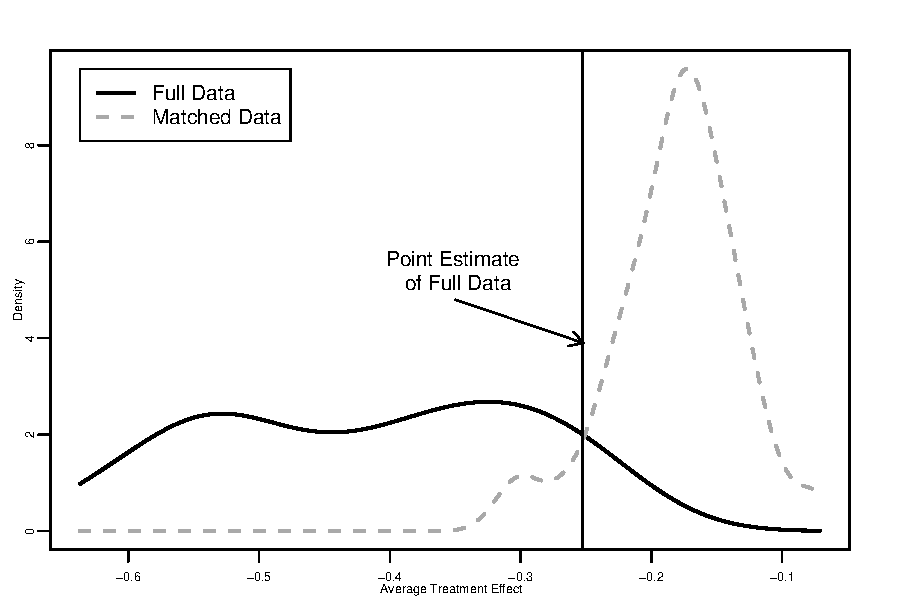
\includegraphics[height=3.5in,angle=0]{dens.pdf}
  \end{center}
  \vspace{-0.275in}
  \caption{Density estimates of estimated effects of being
    a highly visible female Republican candidate across 63 possible
    specifications with the Koch data.  The solid line presents
    estimates for the full dataset and the dashed line presents
    estimates for the matched dataset (via subclassification).  The
    solid vertical line presents the point estimate of the regression
    presented in the original paper.  This figure shows that treatment
    effect estimates are much more sensitive to model specification
    for the full dataset compared to the matched dataset.}
  \label{fg:kochdens}
\end{figure}

\end{document}
